\documentclass{beamer}

\usetheme[]{Rochester}
\usecolortheme{beaver}
\usepackage[latin1]{inputenc}
\usepackage{graphics}

\author{Will Webberley}
\date{Autumn 2014}
\institute[COMSC]{Cardiff School of Computer Science and Informatics}



\title{Design and Usability Principles \& Heuristics}
\subtitle{CM2101: Human-Computer Interaction}

\begin{document}

\frame{\titlepage}

\frame{
    \frametitle{Interaction design principles}
    \begin{itemize}
        \item Concerned with the `physical' interface
        \item Abstractions for thinking about different aspects of design
        \item What to put into an interface and what to leave out
        \item Derived from theory, experience, and common sense
    \end{itemize}
}
 
\frame{
    \frametitle{Design principles}
    \begin{enumerate}
        \item Visibility
        \item Feedback
        \item Constraint
        \item Mapping
        \item Consistency
        \item Affordance
        \item Predictability
        \item Synthesisability
        \item Familiarity
    \end{enumerate}
}

\frame{
    \frametitle{Design principles: Visibility}
    Are available actions visible and obvious? Make relevant parts visible.
    \vskip15pt
    \centering
    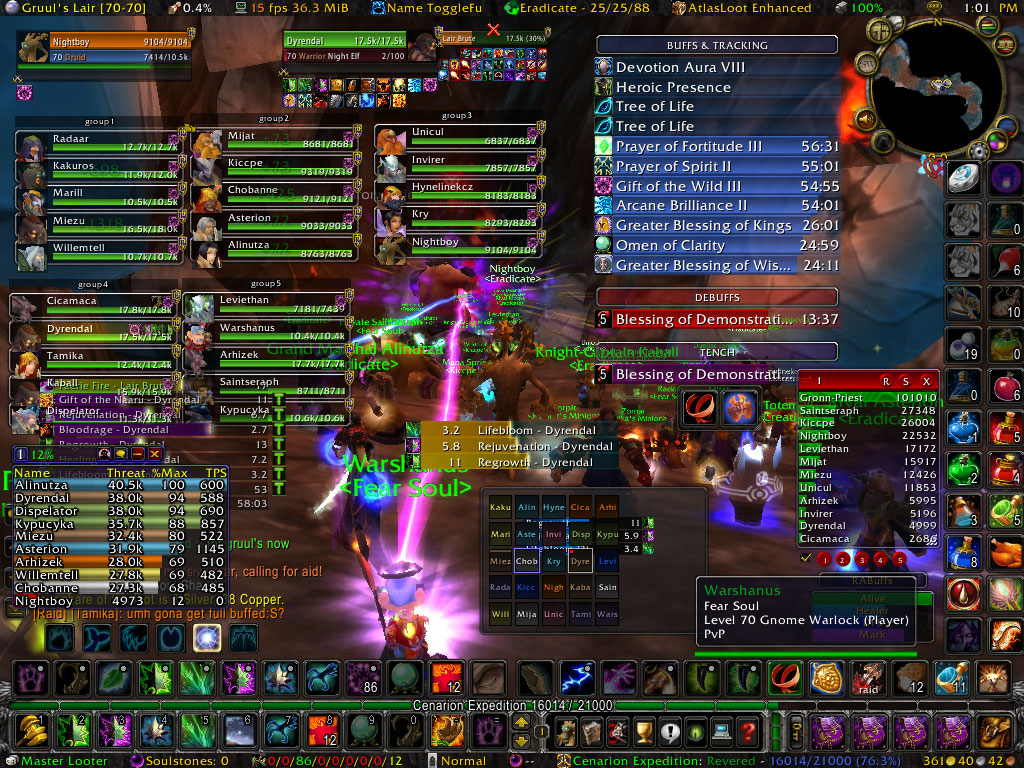
\includegraphics[width=7cm]{media/wow.jpg}    
}   

\frame{
    \frametitle{Design principles: Feedback}
    Update the user on what's going on. Aurally, visibly, physically (e.g. haptic feedback in games, keyboard presses, etc.).
    \vskip15pt
    \centering
    
\includegraphics[width=7cm]{media/progress_bar.png}    
}

\frame{
    \frametitle{Design principles: Constraint}
    \begin{itemize}
        \item Restrict possible actions that can be performed
        \item Stop users from doing things wrong and to help prevent errors 
        \item Types of constraint (Norman 1999)
        \begin{itemize}
            \item Physical
            \item Cultural
            \item Logical
        \end{itemize}
    \end{itemize}
}

\frame{
    \frametitle{Design principles: Constraint}
    \textbf{Physical constraint}
    \begin{columns}
        \column{.5\textwidth}
            \begin{itemize}
                \item The way physical objects restrict movement
                \item How many ways can USB ($<$ v4.0) be inserted?
                \item These constraints prevent physical damage and mistakes from being made.
                \item Bad example: optical media
            \end{itemize}
        \column{.5\textwidth}
            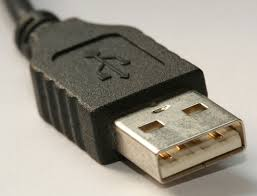
\includegraphics[width=4cm]{media/usb.jpg}
    \end{columns}
}

\frame{
    \frametitle{Design principles: Constraint}
    \textbf{Cultural constraint}
    \begin{columns}
        \column{.5\textwidth}
            \begin{itemize} 
                \item Learned conventions prevent or guide actions
                \item Users can associate components with cultural conventions
                \item Remember that not all cultures have the same conventions
            \end{itemize}
        \column{.5\textwidth}
            
\includegraphics[width=4cm]{media/triangle.png}
    \end{columns}
}

\frame{
    \frametitle{Design principles: Constraint}
    \textbf{Logical constraint}
    \begin{columns}
        \column{.5\textwidth}
            \begin{itemize} 
                \item Rely on common sense and users' ability to be logical
                \item Read indicators 
                \item For example, assume users know not to plug an HDMI cable into a DVI port
                \item Similar examples in software (e.g. know the general form of an email address)
            \end{itemize}
        \column{.5\textwidth}
            
\includegraphics[width=5cm]{media/email.png}
    \end{columns}
}

\frame{
    \frametitle{Design principles: Mapping}
    Relationship between controls and movements in the real-world. Use similar controls for those for similar real-world objects. A bad example of mapping in the real-world is a bank of light switches.
    \vskip15pt
    \centering
    \begin{columns}
        \column{.5\textwidth}
            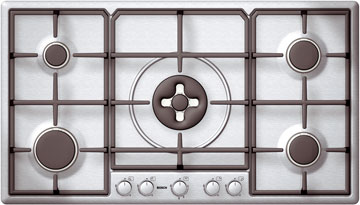
\includegraphics[width=4cm]{media/good_hob.jpg}
        \column{.5\textwidth}
            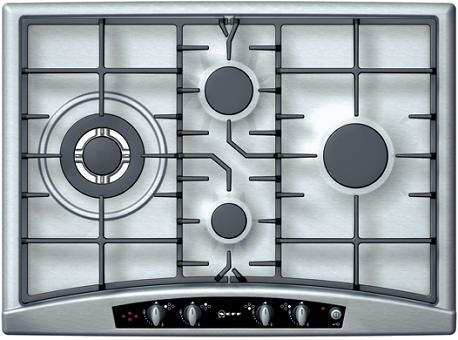
\includegraphics[width=4cm]{media/bad_hob.jpg}
    \end{columns}    
}

\frame{
    \frametitle{Design principles: Consistency}
    \begin{itemize}
        \item Interfaces should use the same words/icons/colours/sounds/experience for the same tasks
        \item Associated tasks should be made clear
        \item Consistent interfaces help with \textit{learnability} (we'll cover this shortly)
        \item The `principles of least surprise'
        \item Types of consistency
        \begin{itemize}
            \item Internal
            \item External
        \end{itemize}
    \end{itemize}
}

\frame{
    \frametitle{Design principles: Consistency}
    \textbf{Internal consistency}
    \begin{columns}
        \column{.5\textwidth}
            \begin{itemize} 
                \item Operations should behave the same within an application
                \item Look and feel should be consistent (e.g. same colour scheme, fonts, text-sizes, etc.)
                \item Use the same terminology (e.g. don't use both `save file' and `write to disk')
                \item Hard in complex situations
            \end{itemize}
        \column{.5\textwidth}
            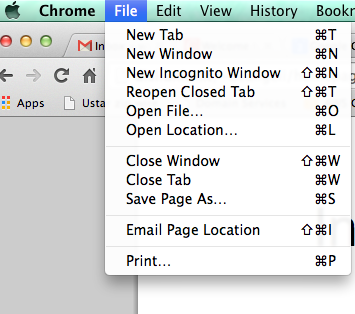
\includegraphics[width=5cm]{media/internal_consistency.png}
    \end{columns}
}

\frame{
    \frametitle{Design principles: Consistency}
    \textbf{External consistency}
    \begin{columns}
        \column{.5\textwidth}
            \begin{itemize} 
                \item Linked to \textit{Mapping}
                \item Design interfaces to be the same across applications and devices
                \item Hard because everyone has different opinions on how things should be done
                \item Often standards are set in various fields to help with this (e.g. W3C)
            \end{itemize}
        \column{.5\textwidth}
            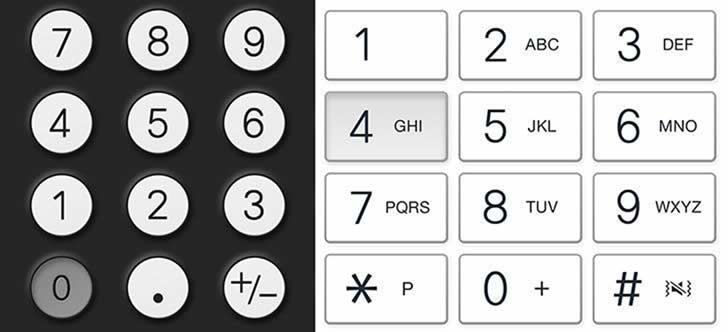
\includegraphics[width=5cm]{media/external_consistency.jpg}
    \end{columns}
}

\frame{
    \frametitle{Design principles: Affordance}
    An attribute of an object that people recognise and know how to use (e.g. `pulling a door handle' and `pressing a button'). Linked to \textit{Mapping}, yet some mappings are better than others! 
    \vskip15pt
    \centering
    
\includegraphics[width=7cm]{media/slider.png}
}            



\frame{
    \frametitle{Revisiting usability}
    \alert{Usability}

    \center{
        \textrm{\textit{
            ``Extent to which a product can be used by 
            specified users to achieve specified goals 
            with \alert{effectiveness}, \alert{efficiency} and 
            \alert{satisfaction} in a specified context of use.''
        }}
    }
    \vskip20pt
    \fontsize{10pt}{12pt}\selectfont
    \flushleft{
        - ISO 9241-11:1998 Part 11: Guidance on usability
    }
}

\frame{
    \frametitle{Revisiting usability}
    \center{
        Design principles are useful for \alert{designing interfaces}.
        \vskip30pt
        Usability principles are useful for \alert{evaluating interactions} and often address the design principles.
    }
    \vskip40pt
    \flushleft{
        Generally, the two sets of principles can be used interchangeably in the design and evaluation of interfaces and interactions.
    }
}

\frame{
    \frametitle{Revisiting usability}
    \center{
        Effectively, usability is a quality attribute that \alert{assesses} how easy interfaces are to use.
    }
    \vskip20pt
    \flushleft{
        Where quality = \alert{absence of problems}         
    }
    \begin{itemize}
        \item Evaluate a system to discover usability problems
        \item Reduce their frequency and severity
        \item Highlighted through \alert{user evaluation} and \alert{heuristic evaluation}
        \item Software designers have a lot to consider (e.g. functionality, performance, cost, security, robustness, usability, etc.)
        \begin{itemize}
            \item However, usability is our main goal in HCI
        \end{itemize}
    \end{itemize}
}

\frame{
    \frametitle{General usability principles}
    \begin{enumerate}
        \item Learnability
        \item Visibility
        \item User control \& memorability 
        \item Errors
        \item Efficiency
        \item Satisfaction 
    \end{enumerate}
    \vskip30pt
    Often address the design principles (given in italics in the following slides).
}

\frame{
    \frametitle{General usability principles: Learnability}
    \alert{How easy is the system to use the first time?\\ How easy is it to learn?}\\
    Types of learnability
    \begin{itemize}
        \item Predictability
        \item Synthesisability
        \item Familiarity
        \item Generalisability
    \end{itemize}
    \vskip30pt
    \begin{columns}
        \column{.4\textwidth}
            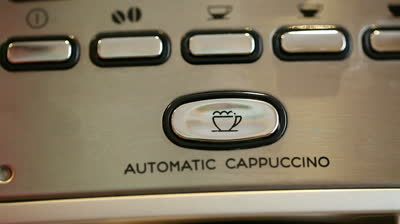
\includegraphics[width=4cm]{media/easy_coffee.jpg}
        \column{.1\textwidth}
            vs.
        \column{.4\textwidth}
            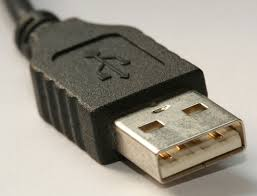
\includegraphics[width=4cm]{media/usb.jpg}
    \end{columns}
}

\frame{
    \frametitle{General usability principles: Learnability}
    \textbf{Predictability}
    \vskip20pt
    Can user predict what will happen if an action is taken? This can be based on \alert{past interaction history}.\\
    For example, should users expect to receive a confirm dialogue when deleting an object?
    \vskip15pt
    \centering
    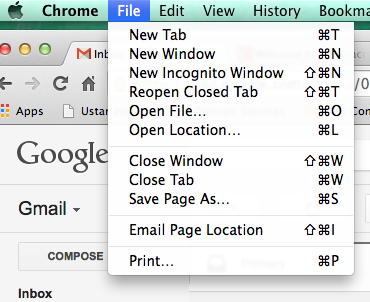
\includegraphics[height=3cm]{media/predictability_1.png}
    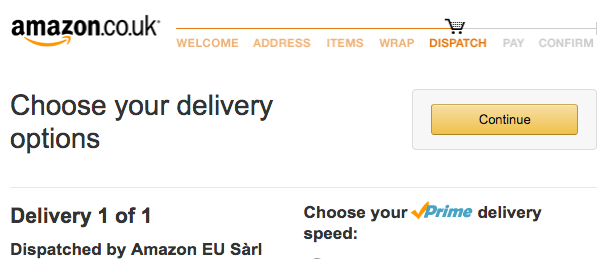
\includegraphics[height=3cm]{media/predictability_2.png}
}

\frame{
    \frametitle{General usability principles: Learnability}
    \textbf{Synthesisability}
    \vskip20pt
    Can the user see the result of an action and assess events of past actions? 
    \begin{itemize}
        \item Linked to \textit{Feedback}
        \item Some interfaces promise \alert{immediate honesty} (i.e. the new state is immediately obvious)
        \item Other interfaces promise \alert{eventual honesty} (i.e. in the case of asynchronous tasks)
    \end{itemize}
}

\frame{
    \frametitle{General usability principles: Learnability}
    \textbf{Familiarity}
    \vskip20pt
    Can user expectation be matched?
    \begin{itemize}
        \item Address \textit{Affordance} by making components feel familiar
        \item Use natural (or domain-specific language)
        \item Address \textit{Predictability} by improving system guessability
    \end{itemize}
}

\frame{
    \frametitle{General usability principles: Learnability}
    \textbf{Generalisability}
    \vskip20pt
    Is it easy to perform new tasks given the user's present knowledge of the system?
    \begin{itemize}
        \item Related to \textit{Consistency} 
        \item For example, if user knows the tool for drawing a square, will they know how to draw a circle?
        \item Offering standard procedures (e.g. copy+paste) also helps this
    \end{itemize}
}

\frame{
    \frametitle{Design principles: Visibility}
    \alert{How visible is the state of the system?}\\
    Addresses the \textit{Visibility} design principle, but more from an \alert{interaction} point of view than just the \alert{interface}.
    \vskip30pt
    \begin{columns}
        \column{.4\textwidth}
            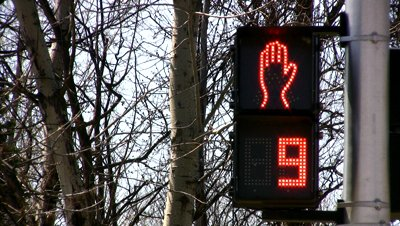
\includegraphics[width=4cm]{media/countdown.jpg}
        \column{.1\textwidth}
            vs.
        \column{.4\textwidth}
            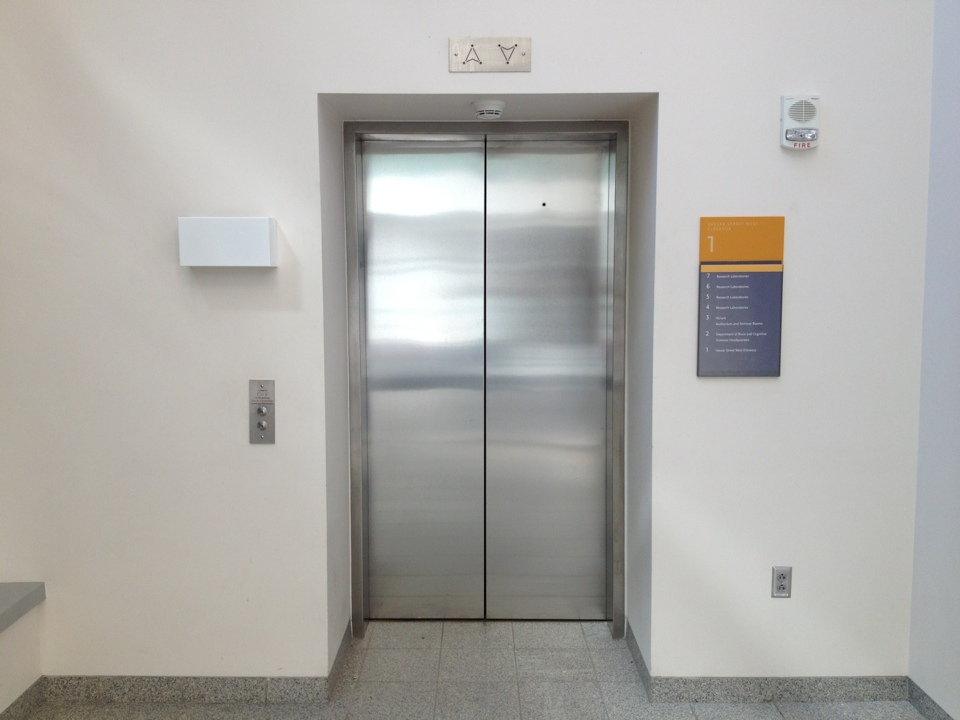
\includegraphics[width=4cm]{media/lift.jpg}
    \end{columns}
}

\frame{
    \frametitle{General usability principles: User control \& memorability}
    \alert{Is user free to explore the system?\\ How easy is it to return to the system after not using it?\\ Are abbreviations and shortcuts appropriate?}
    Human working memory is small and very temporary
    \vskip30pt
    \begin{columns}
        \column{.45\textwidth}
            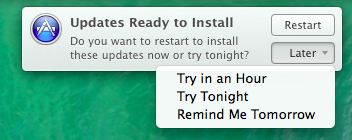
\includegraphics[width=4cm]{media/update.png}
        \column{.1\textwidth}
            vs.
        \column{.45\textwidth}
            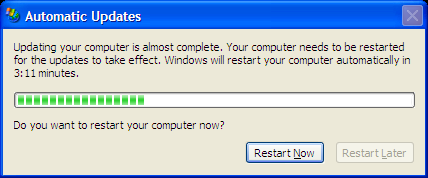
\includegraphics[width=4cm]{media/restart.png}
    \end{columns}
}

\frame{
    \frametitle{General usability principles: Errors}
    \alert{Are errors too easy to make?\\ Are errors easy to recover from?}
    \vskip30pt
    \begin{columns}
        \column{.45\textwidth}
            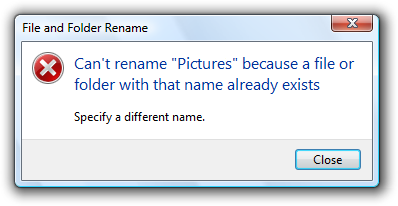
\includegraphics[width=5cm]{media/good_error.png}
        \column{.1\textwidth}
            vs.
        \column{.45\textwidth}
            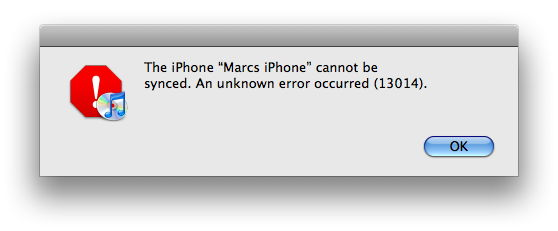
\includegraphics[width=5cm]{media/iphone_error.jpg}
    \end{columns}
}   

\frame{
    \frametitle{General usability principles: Efficiency}
    \alert{Once learned, how quickly can tasks be performed?}
    \begin{itemize}
        \item Can experts gradually use the system faster?
        \item Systems should be elastic to allow this, but also to support less-experienced uers.
    \end{itemize}
}   

\frame{
    \frametitle{General usability principles: Satisfaction}
    \alert{Is the system a pleasure to use?}
    \vskip30pt
    \begin{columns}
        \column{.4\textwidth}
            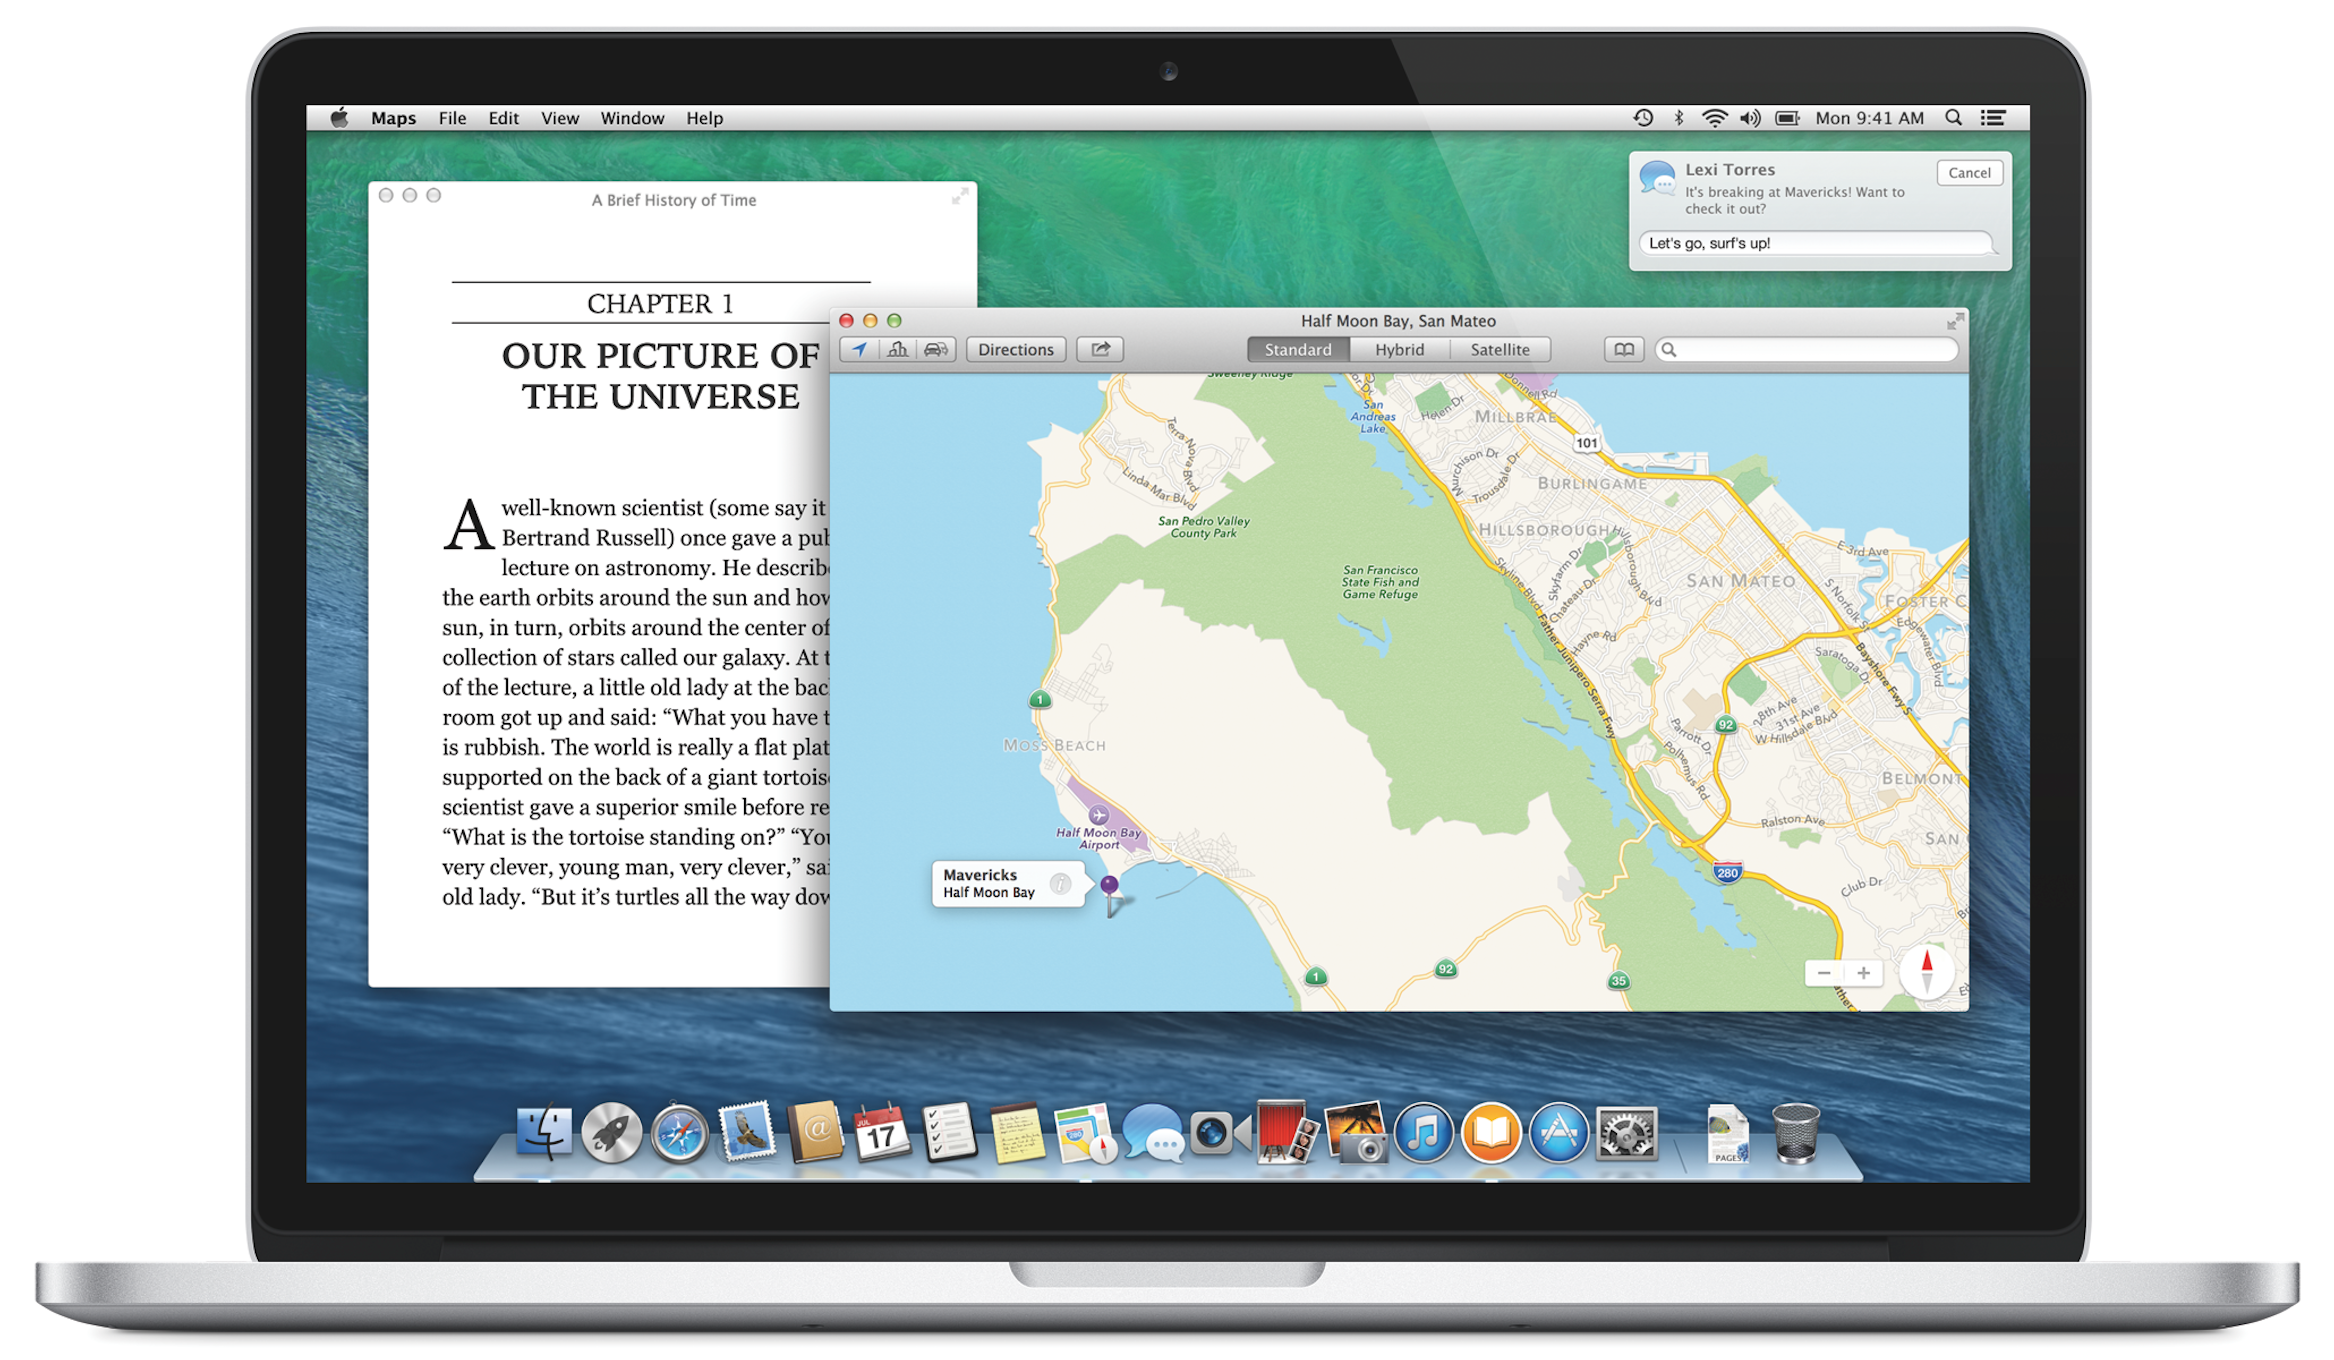
\includegraphics[width=5cm]{media/mavericks.png}
        \column{.1\textwidth}
            vs.
        \column{.4\textwidth}
            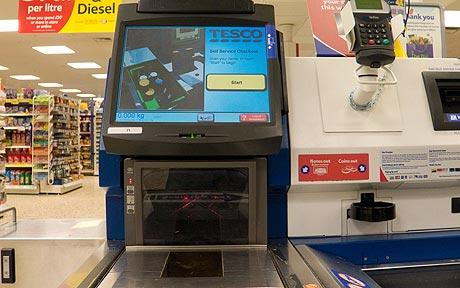
\includegraphics[width=4cm]{media/checkout.jpg}
    \end{columns}
}

\frame{
    \frametitle{General usability principles}
    \begin{itemize}
        \item Systems can be evaluated \alert{with respect to} the principles
        \item When designing interactions, try and \alert{consider all} usability and design principles
        \item Aim of systems should be to \alert{maximise} all
    \end{itemize}
    \vskip20pt
    For some systems, some principles are prioritised more than others.\\
    For example, in iOS, \alert{\textit{Satisfaction}} is considered more highly than the design principle \alert{\textit{Visibility}}. 
}

\frame{
    \frametitle{Design and usability principles}
    \center{
        These principles form the baseline for \alert{Neilsen's heuristics}.
    }
    \vskip20pt
    `Heuristics' are broad rules of thumb. Neilsen's heuristics are not specific usability guidelines, but are useful for evaluating systems.
}

\frame{
    \frametitle{Neilsen's heuristics}
    \begin{enumerate}
        \item Visibility of system status
        \begin{itemize}
            \item System should inform users about what's going on internally.
        \end{itemize}
        \item Match between system and real world
        \begin{itemize}
            \item System should speak the user's language and allow functions in a logical order.
        \end{itemize}
        \item User control and freedom
        \begin{itemize}
            \item Provide an `emergency exit' (e.g. by allowing an `undo' action)
        \end{itemize}
        \item Consistency and standards
        \begin{itemize}
            \item Ensure that different words or actions don't mean the same thing. Follow the platform guidelines.
        \end{itemize}
        \item Error prevention
        \begin{itemize}
            \item As well as using good error messages, try and prevent errors from happening.
        \end{itemize}
    \end{enumerate}
}

\frame{
    \frametitle{Neilsen's heuristics}
    \begin{enumerate}
        \setcounter{enumi}{5}
        \item Recognition rather than recall
        \begin{itemize}
            \item Reduce users' memory loads by making actions and options visible. Use standard practices.
        \end{itemize}
        \item Flexibility and efficiency
        \begin{itemize}
            \item Cater to both expert and unexperienced users by making it faster to use for experts.
        \end{itemize}
        \item Aesthetic and minimalist design
        \begin{itemize}
            \item Do not display irrelevant information. Keep interface concise and provide contextually relevant actions.
        \end{itemize}
        \item Help users recognise, diagnose, and recover from errors
        \begin{itemize}
            \item Use English, avoid error codes, constructively provide a solution.
        \end{itemize}
        \item Help and documentation
        \begin{itemize}
            \item If you \textit{do} need documentation, make it easily searchable and task-focussed.
        \end{itemize}
    \end{enumerate}
}

\frame{
    \frametitle{Revision questions}
    \begin{enumerate}
        \item What are design principles and why are they useful?
        \item Name and describe three types of constraint when considering design principles.
        \item Why is mapping between systems and the real-world important?
        \item What is external consistency and describe a way in which it can be addressed?
        \item As well as by \textit{frequency}, in which other way should usability problems be reduced?
        \item Give an example of a system where \textit{visibility} is not considered as a usability principle.
        \item Describe a way in which you might help reduce errors occurring in a system.
        \item Describe what is meant by the \textit{user control \& memorability} usability principle.
    \end{enumerate}
}

\frame{
    \frametitle{Summary}
    \begin{itemize}
        \item Introduction and description of the general \alert{design principles}
        \item Overview of the general \alert{usability principles}
        \item Identified use of both types of principles
        \item Introduction to Neilsen's heuristics 
    \end{itemize}
}

\end{document}
